\documentclass[12pt]{exam}
\usepackage[
  letterpaper,
  margin=0.3in,
  includehead,    % include the header area in the 0.25in margin
  includefoot     % include the footer area in the 0.25in margin
]{geometry}
\usepackage[shortlabels]{enumitem}
\setlist[enumerate,1]{label=(\alph*)} %makes list alphabetic

\usepackage{physics}

\usepackage{pgfplots} % For sketching graphs
\pgfplotsset{compat=1.18}


\usepackage{caption}

\title{Introduction to Quantum Mechanics - Solution Manual \newline \small{For Griffiths and Schroeter's Third Edition}}

\author{Justin Beltran}
\date{May 2025}

\begin{document}

\maketitle
\firstpagefooter{}{}{By Justin Beltran}
\runningfooter{}{}{By Justin Beltran}
\printanswers

\section{Chapter 1}



\subsection*{Problem 1.1}
For the distribution of ages in the example in Section 1.3.1
\begin{enumerate}[(a)]
    \item  Compute $\expval{j^2}$ and $\expval{j}^2$

    \item Determine $\Delta j$ for each $j$, and use Equation 1.11 to compute the standard deviation.

    \item Use your results in (a) and (b) to check Equation 1.12
\end{enumerate}

\begin{solution}
    \begin{enumerate}[(a)]
        \item There is one person aged 14, one person aged 15, three people aged 16, two people aged 22, two people aged 24, five people aged 25 then 
        $$\expval{j^2} = \sum_j j^2 P(j) = 14^2(\frac{1}{14}) + 15^2(\frac{1}{14}) + 16^2(\frac{3}{14})+ 22^2(\frac{2}{14})+ 24^2(\frac{2}{14})+ 25^2(\frac{5}{14})$$
        $$= \frac{196}{14} + \frac{225}{14}+ \frac{768}{14}+ \frac{968}{14}+ \frac{1152}{14}+ \frac{3125}{14} = \frac{6434}{14} = 459.57$$
        and 
        $$\expval{j}^2 =  \big[\sum_j j^ P(j) = 14(\frac{1}{14}) + 15(\frac{1}{14}) + 16(\frac{3}{14})+ 22(\frac{2}{14})+ 24(\frac{2}{14})+ 25(\frac{5}{14})\big]^2$$
        $$= \big[ \frac{14}{14}+ \frac{15}{14} + \frac{48}{14} + \frac{44}{14} + \frac{48}{14} + \frac{125}{14}\big]^2 = \big[\frac{294}{14}\big]^2 = 21^2 = 441$$

        \item $\expval{j}=21$ then $\Delta j_{14} = 14-21 = -7$, $\Delta j_{15} = 15-21 = -6$, $\Delta j_{16} = 16-21 = -5$,  $\Delta j_{22} = 22-21 = 1$, $\Delta j_{24} = 24-21 = 3$, $\Delta j_{25} = 25-21 = 4$.  Plugging into 1.11 $$\sigma^2 = \expval{(\Delta j)^2}  = (-7)^2(\frac{1}{14}) + (-6)^2(\frac{1}{14}) + (-5)^2(\frac{3}{14})+ 1^2(\frac{2}{14})+ 3^2(\frac{2}{14})+ 4^2(\frac{5}{14})$$ 
        $$
        = 49(\frac{1}{14}) + 36(\frac{1}{14}) + 25(\frac{3}{14})+ (\frac{2}{14})+ 9(\frac{2}{14})+ 16(\frac{5}{14})= \frac{259}{14} = 18.57 \implies\sigma = 4.31$$

        \item Equation 1.12 states $\sigma = \sqrt{\expval{j^2}-\expval{j}^2}$ so plugging in answers from part (a) yields $\sigma =\sqrt{459.57-441} = 18.57$ which is as expected.
    \end{enumerate}
\end{solution}


\subsection*{Problem 1.2}
\begin{enumerate}[(a)]
    \item Find the standard deviation of the distribution in Example 1.2.


    \item What is the probability that a photograph, selected at random, would show a distance $x$ more than one standard deviation away from the average?
\end{enumerate}

\begin{solution}
    \begin{enumerate}[(a)]
        \item Noting that $\expval{x} = \frac{h}{3}$ then $\expval{x}^2 = \frac{h^2}{9}$. Now computing $\expval{x^2} = \int x^2\rho (x)dx$ with $\rho(x) = \frac{1}{2\sqrt{hx}} \implies$
        $$\expval{x^2} = \int^h_0 x^2 \frac{1}{h\sqrt{2x}} dx = \frac{1}{h\sqrt{2}} \int^h_0 x^{1.5}dx =  \frac{1}{h\sqrt{2}} \frac{1}{2.5} x^{2.5} \bigg|^h_0 = \frac{1}{5}h^2$$ plugging it all into $\sigma = \sqrt{\expval{j^2}-\expval{j}^2}$  gives 
        $$\sigma = \sqrt{\frac{h^2}{5}-\frac{h^2}{9}} = \sqrt{\frac{4h^2}{45}} = \frac{2h}{\sqrt{45}}$$

        \item Since the probability of finding the rock is a non-uniform distribution, consider the whole probability subtracted by the probability of being within one standard deviation 
        $$P = 1 - \int^{\expval{x}+\sigma}_{\expval{x}-\sigma} \frac{1}{2\sqrt{hx}}dx = 1-  \frac{1}{2\sqrt{h}}\int^{\expval{x}+\sigma}_{\expval{x}-\sigma} \frac{1}{\sqrt{x}}dx = 1- \frac{1}{2\sqrt{h}}\bigg[2\sqrt{x}\big|^{\expval{x}+\sigma}_{\expval{x}-\sigma}\bigg]$$
        $$=  1- \frac{1}{\sqrt{h}}\bigg[ \sqrt{\expval{x}+\sigma} - \sqrt{\expval{x}-\sigma}\bigg] \text{plugging in} = 1 - \frac{1}{\sqrt{h}}\bigg[ \sqrt{\frac{h}{3}+\frac{2h}{\sqrt{45}}} - \sqrt{\frac{h}{3}-\frac{2h}{\sqrt{45}}}\bigg]$$
        $$ = 1 - 0.795 + 0.188 = 0.393 = 39.3\%$$
    \end{enumerate}
\end{solution}



\subsection*{Problem 1.3}
Consider the \textbf{gaussian} distribution $\rho(x) = Ae^{-\lambda(x-a)^2}$ where $A$, $a$, and $\lambda$ are positive real constants. (The necessary integrals ae inside the back cover.)
\begin{enumerate}[(a)]
    \item Use Equation 1.16 to determine $A$.
    \item Find $\expval{x}, \expval{x^2}$, and $\sigma$.
    \item Sketch the graph of $\rho(x)$
\end{enumerate}

\begin{solution}
    \begin{enumerate}[(a)]
        \item Equation 1.16 states $1 = \int^\infty_{-\infty} \rho(x)dx$ so plugging in 
        $$1 =\int^\infty_{-\infty} Ae^{-\lambda(x-a)^2}dx = A \int^\infty_{-\infty} e^{-\lambda(x-a)^2}dx$$ 
        now let $u = x-a $ then $du = dx$ 
        $$1 =A\int^\infty_{-\infty} e^{-\lambda(u)^2}du = A\frac{1}{\sqrt\lambda}\sqrt{\pi} \implies A = \sqrt{\frac{\lambda}{\pi}}$$

        \item First $$\expval{x} = A \int^\infty_{-\infty} xe^{-\lambda(x-a)^2} dx \text{ let $u = x-a$ then } = A \int^\infty_{-\infty} (u+a)e^{-\lambda(u)^2} du $$
        and let $w = -\lambda u^2$ then $du =\frac{dw}{-\lambda2u}$
        
        $$= A \bigg[\frac{-1}{2\lambda}\int^\infty_{-\infty} e^{w} dw + a\int^\infty_{-\infty} e^{-\lambda u^2} du\bigg] = A\bigg[ \frac{-1}{2\lambda}e^{-\lambda u}\big|^\infty_{-\infty} + a\sqrt{\frac{\pi}{\lambda}} \bigg] = Aa\sqrt{\frac{\pi}{\lambda}} = a$$

        Now computing $\expval{x^2}$  $$\expval{x^2} = A \int^\infty_{-\infty} x^2e^{-\lambda(x-a)^2} dx \text{ let $u = x-a$ then } = A \int^\infty_{-\infty} (u+a)^2e^{-\lambda u^2} du $$
        
        $$\int^\infty_{-\infty} (u^2 + 2au +a^2)e^{-\lambda u^2}du = \int^\infty_{-\infty} u^2 e^{-\lambda u^2}du + 2a\int^\infty_{-\infty}ue^{-\lambda u^2}du + a^2\int^\infty_{-\infty}e^{-\lambda u^2}du$$
        where the right two integrals on the RHS were already computed thus
        $$A\int^\infty_{-\infty} (u+a)^2e^{-\lambda u^2}du  = A\bigg[\int^\infty_{-\infty} u^2 e^{-\lambda u^2}du + 0 + a^2\sqrt{\frac{\pi}{\lambda}} \bigg]$$
        $$ = A\bigg[ 2\sqrt{\pi}2!\big(\frac{1}{2\sqrt{\lambda}}\big)^3 + a^2 \sqrt{\frac{\pi}{\lambda}} \bigg] = A\sqrt{\frac{\pi}{\lambda}} \bigg(\frac{1}{2\lambda} +a^2\bigg) = \frac{1}{2\lambda} +a^2$$

        Lastly calculating $\sigma = \sqrt{\expval{j^2}-\expval{j}^2}$ gives 
        $$\sigma = \sqrt{ \bigg(\frac{1}{2\lambda} +a^2\bigg) - \big(a\big)^2} = \frac{1}{2\lambda}$$

        \item Note that the peak occurs around $x = a$, $\lambda$ controls the stiffness of the peak, and $A$ controls the amplitude. 

        \noindent

        \begin{minipage}[t]{0.45\textwidth}
          \centering
          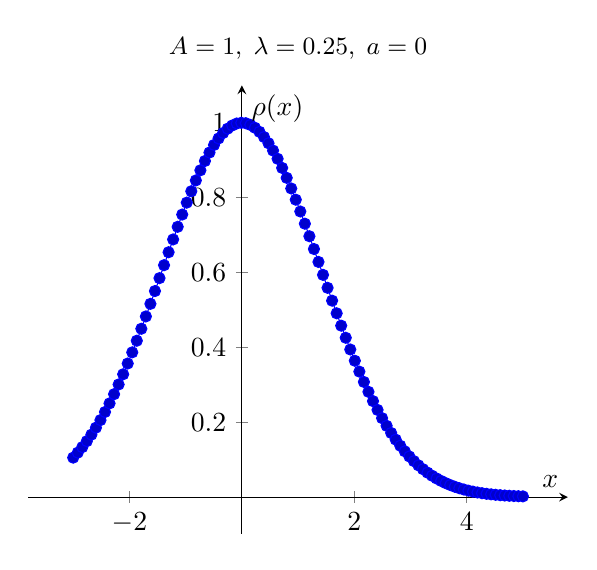
\begin{tikzpicture}
            \begin{axis}[
              domain=-3:5, samples=100,
              xlabel={$x$}, ylabel={$\rho(x)$},
              axis lines=middle, enlargelimits=0.1,
              title={$A=1,\;\lambda=0.25,\;a=0$},  
              title style={font=\small}
            ]
              \addplot {exp(-0.25*(x)^2)};
            \end{axis}
          \end{tikzpicture}
        \end{minipage}\hfill
        \begin{minipage}[t]{0.48\textwidth}
          \centering
          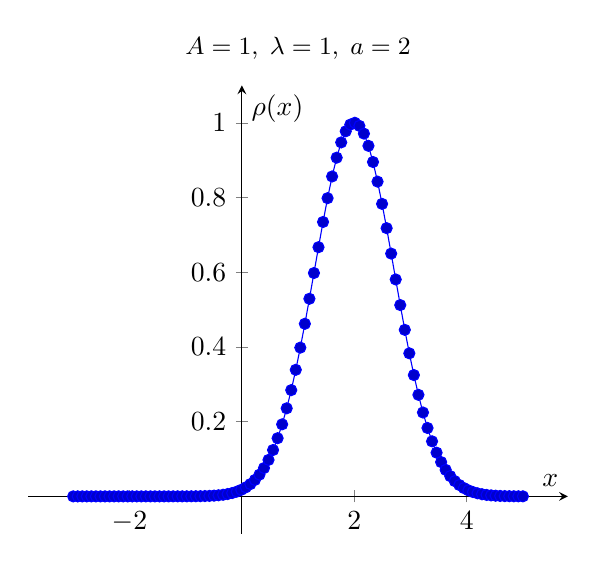
\begin{tikzpicture}
            \begin{axis}[
              domain=-3:5, samples=100,
              xlabel={$x$}, ylabel={$\rho(x)$},
              axis lines=middle, enlargelimits=0.1,
              title={$A=1,\;\lambda=1,\;a=2$},  
              title style={font=\small}
            ]
              \addplot {1*exp(-1*(x-2)^2)};
            \end{axis}
          \end{tikzpicture}
        \end{minipage}

    \end{enumerate}
\end{solution}


\subsection*{Problem 1.4}
At time $t=0$ a particle is represented by the wave function \[
\psi(x)=
\begin{cases}
  A(x/a),            & 0 \le x \le a,\\
  A(b-x)/(b-a),              & a \le x \le b.
\end{cases}
\] 
and $0$ otherwise, where $A$, $a$, and $b$ are positive constants.
\begin{enumerate}
    \item Normalize $\Psi$ (that is, find $A$ in terms of $a$ and $b$).
    \item Sketch $\Psi(x,0)$, as a function of $x$.
    \item Where is the particle most likely to be found, at $t=0$?
    \item What is the probability of finding the particle to the left of $a$? Check your result in the limiting cases $b=a$ and $b=2a$.
    \item What is the expectation value of $x$?
\end{enumerate}

\begin{solution}
    \begin{enumerate}
        \item Beginning with $\int |\Psi(x,t)|^2dx =1$ split the integral over the two different cases of $\Psi$ that is
        $$1 = \int^b_a \bigg|A\frac{(b-x)}{(b-a)}\bigg|^2dx + \int^a_0 \bigg|A\frac{x}{a}\bigg|^2 = 
        \bigg|\frac{A}{(b-a)}\bigg|^2\int^b_a (b-x)^2dx + \bigg|\frac{A}{a}\bigg|^2\int^a_0 x^2 dx
        $$
        $$=-\bigg|\frac{A}{(b-a)}\bigg|^2\frac{1}{3}(b-x)^3\big|^b_a + \bigg|\frac{A}{a}\bigg|^2\frac{1}{3}x^3\big|^a_0=\bigg|\frac{A}{(b-a)}\bigg|^2\frac{1}{3}(b-a)^3 + \bigg|\frac{A}{a}\bigg|^2\frac{1}{3}a^3\implies$$
        $$3 = \frac{|A|^2}{|b-a|^2}(b-a)^3 + \frac{|A|^2}{|a|^2}a^3 = |A|^2(b-a) +|A|^2a \implies$$
        $$ 3 = |A|^2b \implies A = \sqrt{\frac{3}{b}}$$
        
        \item Let $A=1$ so the max amplitude is 1 (this is arbitrary, its just to note the peak is at $A$). Really the area under the blue and red line should sum to 1. 
        
        \noindent
        \begin{minipage}[t]{0.48\textwidth}
          \centering
          \begin{tikzpicture}
            %--- parameters:
            \pgfmathsetmacro{\A}{1}   % amplitude
            \pgfmathsetmacro{\a}{2}   % left knot
            \pgfmathsetmacro{\b}{6}   % right knot
        
            \begin{axis}[
              domain=0:\b,
              samples=100,
              xlabel={$x$}, ylabel={$\psi(x)$},
              axis lines=middle,
              enlargelimits=0.1,
              ymin=0,
              xtick={0,\a,\b},
              xticklabels={$0$,$a$,$b$},
              legend pos=outer north east,
            ]
              % 1) branch on [0,a]
              \addplot[blue, thick, domain=0:\a] { \A*(x/\a) };
              \addlegendentry{$0\le x\le a$}
        
              % 2) branch on [a,b]
              \addplot[red, thick, domain=\a:\b] { \A*((\b - x)/(\b - \a)) };
              \addlegendentry{$a\le x\le b$}
            \end{axis}
          \end{tikzpicture}
        \end{minipage}

        \item The particle is most likely to be found at $x=a$ for $t=0$.

        \item The probability of finding the particle left of $a$ is given by the area under the blue line so 
        $$P[x<a] = \frac{A^2}{a^2}\int^a_0 x^2dx =  \frac{A^2}{a^2}\frac{a^3}{3}  = \frac{3}{b}\frac{a}{3}=\frac{a}{b}$$ and note when $b=a$ there is probablity 1 i.e. guranteed to find. When $b=2a$ (the midpoint) its $\frac{1}{2}$ as expected.

        \item EV for $x$ is given by $\expval{x} = \int x \rho(x)dx$ where $|\Psi(x,t)|^2$ is the probability density, $\rho(x)$, since $\Psi$ is 0 outside the bounds by the vanishing theorem the integral reduces to   
        $$\expval{x} = \int^b_0 x|\Psi|^2dx = \int^b_a x\bigg|A\frac{(b-x)}{(b-a)}\bigg|^2dx + \int^a_0 x\bigg|A\frac{x}{a}\bigg|^2dx = \bigg|\frac{A}{(b-a)}\bigg|^2\int^b_a x(b-x)^2dx + \bigg|\frac{A}{a}\bigg|^2\int^a_0 x^3 dx$$
        $$=\frac{|A|^2}{|b-a|^2}\bigg[-\frac{x}{3}(b-x)^3 -\frac{1}{12}(b-x)^4\bigg]^b_a + \frac{|A|^2}{|a|^2}\frac{x^4}{4}\bigg|^a_0 = \frac{|A|^2}{|b-a|^2}\bigg[\frac{a}{3}(b-a)^3 +\frac{1}{12}(b-a)^4\bigg] + \frac{|A|^2}{|a|^2}\frac{a^4}{4}$$
        $$=|A|^2 \bigg[\frac{a}{3}(b-a) +\frac{1}{12}(b-a)^2 + \frac{a^2}{4}\bigg] = \frac{3}{b} \bigg[\frac{ab}{3}-\frac{a^2}{3} +\frac{b^2}{12}-\frac{2ab}{12} +\frac{a^2}{12} + \frac{a^2}{4}\bigg] = a + \frac{b}{4}-\frac{a}{2} \implies$$
        $$\expval{x} = \frac{b}{4}+\frac{a}{2}$$
    \end{enumerate}
\end{solution}



\subsection*{Problem 1.5}
Consider the wave function $\Psi(x,t) = Ae^{-\lambda|x|}e^{-i\omega t}$ where $A$, $\lambda$, and $\omega$ are positive real constants. (We'll see in Chapter 2 for what potential (v) this wave function satisfies the Schrodinger equation.)
\begin{enumerate}
    \item Normalize $\Psi$.
    \item Determine the expectation values of $x$ and $x^2$.
    \item Find the standard deviation of $x$. Sketch the graph of $|\Psi|^2$, as a function of $x$ and mark the points $(\expval{x}+\sigma)$ and $(\expval{x}-\sigma)$, to illustrate the sense in which $\sigma$ represents the "spread" in $x$. What is the probability that the particle would be found outside this range?
\end{enumerate}

\begin{solution}
    \begin{enumerate}
        \item Take $\int |\Psi(x,t)|^2dx =1$ and fold the integral over 0 (allowed by symmetry of $\Psi$) otherwise the solution goes to $\infty$ which cannot be since the probability is bounded by 1. 
        $$1=2\int^\infty_0 |\Psi(x,t)|^2dx = 2\int^\infty_0 \bigg|Ae^{-\lambda|x|}e^{-i\omega t}\bigg|^2dx = 2|A|^2\int^\infty_0 e^{-\lambda|x|}e^{-i\omega t} \cdot\big(e^{-\lambda|x|}e^{-i\omega t}\big)^*dx$$
        $$= 2|A|^2\int^\infty_0 e^{-\lambda|x|}e^{-i\omega t} e^{-\lambda|x|}e^{i\omega t}dx = 2|A|^2\int^\infty_0 e^{-2\lambda|x|} dx  = 2|A|^2\frac{-1}{2\lambda}e^{-2\lambda|x|} \bigg|^\infty_0 = \frac{|A|^2}{\lambda}$$
        $$1=\frac{|A|^2}{\lambda}\implies A = \sqrt{\lambda}$$

        \item EV for $x$ is given by $\expval{x} = \int x \rho(x)dx = \int x |\Psi|^2dx$ so expanding yields 
        $$\expval{x} = \int^\infty_{-\infty} x|\Psi(x,t)|^2dx = \int^\infty_{-\infty} x\bigg |Ae^{-\lambda|x|} e^{-i\omega t}\bigg|^2dx = |A|^2\int^\infty_{-\infty} xe^{-\lambda|x|}e^{-i\omega t} \cdot\big(e^{-\lambda|x|}e^{-i\omega t}\big)^*dx$$
        $$= |A|^2\int^\infty_{-\infty} xe^{-\lambda|x|}e^{-i\omega t} e^{-\lambda|x|}e^{i\omega t}dx = |A|^2\int^\infty_{-\infty} xe^{-2\lambda|x|} dx = |A|^2 \bigg[-\frac{x}{2\lambda}e^{-2\lambda|x|} - \frac{1}{4\lambda^2}e^{-2\lambda|x|}\bigg]^\infty_{-\infty} = 0$$
        since the $e^{-2\lambda|x|}$ dominates when the limits at $\pm \infty$ are taken. Next EV for $x^2$ is given by $\expval{x^2} = \int x^2 \rho(x)dx$ a similar expansion gives
         $$\expval{x^2} = \int^\infty_{-\infty} x^2|\Psi(x,t)|^2dx = \int^\infty_{-\infty} x^2\bigg |Ae^{-\lambda|x|} e^{-i\omega t}\bigg|^2dx = |A|^2\int^\infty_{-\infty} x^2e^{-\lambda|x|}e^{-i\omega t} \cdot\big(e^{-\lambda|x|}e^{-i\omega t}\big)^*dx$$
        $$= |A|^2\int^\infty_{-\infty} x^2e^{-\lambda|x|}e^{-i\omega t} e^{-\lambda|x|}e^{i\omega t}dx = |A|^2\int^\infty_{-\infty} x^2e^{-2\lambda|x|} dx \text{ folding the integral since its an}$$
        $$\text{even function }= 2|A|^2 \bigg[-\frac{x^2}{2\lambda}e^{-2\lambda|x|} - \frac{2x}{4\lambda^2}e^{-2\lambda|x|} -\frac{2}{8\lambda^3}e^{-2\lambda|x|}\bigg]^\infty_0 = 2|A|^2\frac{2}{8\lambda^3} = \frac{1}{2\lambda^2}$$

        \item The standard dev is given by $\sigma = \sqrt{\expval{j^2}-\expval{j}^2}$ then plugging in yields
        $$\sigma = \sqrt{\expval{x^2}-\expval{x}^2} = \sqrt{\frac{1}{2\lambda^2}-0^2}=\sqrt{\frac{1}{2\lambda^2}}$$ 

        
      \noindent
        
        \begin{minipage}[t]{0.45\textwidth}
        \vspace{0pt}
        \centering
            \begin{tikzpicture}
                %=== choose numerical values for illustration:
                \pgfmathsetmacro{\A}{1}       % amplitude A
                \pgfmathsetmacro{\lam}{1}     % lambda
                % compute sigma = 1/(sqrt(2)*lambda)
                \pgfmathsetmacro{\sig}{1/(sqrt(2)*\lam)}
            
                \begin{axis}[
                  width=1\linewidth,
                  height=0.5\linewidth,
                  domain=-4:4,
                  samples=200,
                  xlabel={$x$},
                  ylabel={$|\Psi|^2$},
                  axis lines=middle,
                  enlargelimits=0.15,
                  ymin=0,
                  xtick={-2,0,2, -\sig,\sig},
                  xticklabels={$-2$,$0$,$2$,$-\sigma$,$\sigma$},
                  ylabel style={anchor=south},
                  clip=false,
                ]
                  % Plot |Psi|^2 = A^2 exp(-2λ|x|)
                  \addplot[thick,blue] {(\A^2)*exp(-2*\lam*abs(x))};
            
                  % dashed vertical lines at x=±σ
                  \draw[dashed] (axis cs:-\sig,0) -- (axis cs:-\sig,{\A^2*exp(-2*\lam*abs(-\sig))});
                  \draw[dashed] (axis cs: \sig,0) -- (axis cs: \sig,{\A^2*exp(-2*\lam*abs(\sig))});
            
                  % annotate the points
                  \node[above] at (axis cs:-\sig,{\A^2*exp(-2*\lam*abs(-\sig))})
                    {};
                  \node[above] at (axis cs: \sig,{\A^2*exp(-2*\lam*abs(\sig))})
                    {};
                \end{axis}
              \end{tikzpicture}
        \end{minipage}\hfill
        \begin{minipage}[t]{0.45\textwidth}
        
        \vspace{0pt}
            The probability of finding the particle outside this range is given by 
            $$P = 2\int^\infty_\sigma |\Psi(x,t)|^2dx \text{ by (a) }$$
            $$= 2|A|^2\frac{-1}{2\lambda}e^{-2\lambda|x|} \bigg|^\infty_\sigma = e^{-2\lambda\sigma}=e^{-\sqrt{2}}$$
        \end{minipage}
    \end{enumerate}
\end{solution}



\subsection*{Problem 1.6}
Why can't you do integration-py-parts directly on the middle expression in Equation 1.29-pull the time derivative over onto $x$, note that $\frac{dx}{dt}=0$, and conclude that $d\expval{x}/dt=0$?

\begin{solution}
    Equation 1.29 states $\frac{d\expval{x}}{dt} = \int x\frac{d}{dt}|\Psi|^2dx$ with the the third expression omitted. Previously in Equation 1.28 $\expval{x}$ is defined as 
    $$ \expval{x}  = \int x|\Psi|^2dx \implies \frac{d}{dt}\expval{x} = \int \frac{d}{dt}\bigg[x|\Psi|^2\bigg]dx \implies \frac{d\expval{x}}{dt} = \int \frac{dx}{dt}|\Psi|^2 + x\frac{d}{dt}|\Psi|^2dx.$$
    Where $d/dt$ is passed through the integral and the product rule is taken and note that $dx/dt = 0$ so that term drops, confirming Equation 1.29. However integration by parts is not allowed because the differentiation is w.r.t $t$ and the integrand would be w.r.t $x$ and these would need to be the same.
\end{solution}



\subsection*{Problem 1.7}
Calculate $d\expval{p}/dt$. \textit{Answer:} $\frac{d\expval{p}}{dt} = \expval{-\frac{dV}{dx}}$. This is an instance of \textbf{Ehrenfest's theorem}, which asserts that \textit{expectation values obey the classical laws}. 

\begin{solution}
    $$\expval{p} = m\frac{d\expval{x}}{dt} = -i\hbar \int \big(\Psi^*\frac{d\Psi}{dx}\big)dx \implies \frac{d}{dt}\expval{p} = -i\hbar \int \frac{d}{dt}\big(\Psi^*\frac{d\Psi}{dx}\big)dx = -i\hbar \int \bigg(\frac{d\Psi^*}{dt}\frac{d\Psi}{dx} + \Psi^*\frac{d^2\Psi}{dxdt}\bigg)dx$$
    
    Now note $\frac{d\Psi}{dt} = \frac{i\hbar}{2m}\frac{d^2\Psi}{dx^2} - \frac{i}{\hbar}V\Psi$ and the complex conjugate is $\frac{d\Psi^*}{dt} = \frac{-i\hbar}{2m}\frac{d^2\Psi^*}{dx^2} + \frac{i}{\hbar}V\Psi^*$ plugging both in gives
    $$\frac{d\expval{p}}{dt} = -i\hbar \int \bigg(\bigg[\frac{-i\hbar}{2m}\frac{d^2\Psi^*}{dx^2} + \frac{i}{\hbar}V\Psi^*\bigg]\frac{d\Psi}{dx} + \Psi^*\frac{d}{dx}\bigg[\frac{i\hbar}{2m}\frac{d^2\Psi}{dx^2} - \frac{i}{\hbar}V\Psi\bigg]\bigg)dx $$
    $$= -i\hbar \int \bigg(\frac{-i\hbar}{2m}\frac{d^2\Psi^*}{dx^2}\frac{d\Psi}{dx} + \frac{i}{\hbar}V\Psi^*\frac{d\Psi}{dx} + \Psi^*\frac{d}{dx}\frac{i\hbar}{2m}\frac{d^2\Psi}{dx^2} - \Psi^*\frac{d}{dx}\frac{i}{\hbar}V\Psi\bigg)dx$$
    
    $$= -i\hbar \int \frac{-i\hbar}{2m}\frac{d^2\Psi^*}{dx^2}\frac{d\Psi}{dx} dx -i\hbar \int \Psi^*\frac{i\hbar}{2m}\frac{d^3\Psi}{dx^3} dx  -i\hbar \int\frac{i}{\hbar}\bigg[V\Psi^*\frac{d\Psi}{dx}   - \Psi^*\frac{d}{dx}V\Psi\bigg]dx$$

    $$=  \frac{-\hbar^2}{2m}\int \frac{d^2\Psi^*}{dx^2}\frac{d\Psi}{dx}dx + \frac{\hbar^2}{2m}\int\Psi^*\frac{d^3\Psi}{dx^3} dx + \int\bigg[V\Psi^*\frac{d\Psi}{dx}   - \Psi^*\frac{dV}{dx}\Psi -\Psi^*V\frac{d\Psi}{dx}\bigg]dx$$ 
    since $\Psi*$ and $\Psi$ vanish at $\pm \infty$ two integration-by-parts yields
    
    $$=  \frac{-\hbar^2}{2m}\int \frac{d^2\Psi^*}{dx^2}\frac{d\Psi}{dx}dx + \frac{\hbar^2}{2m} \bigg[\int \frac{d^2\Psi^*}{dx^2}\frac{d\Psi}{dx}dx - \Psi^*\frac{d^2\Psi}{dx^2}\bigg|^\infty_{-\infty} + \frac{d\Psi^*}{dx}\frac{d\Psi}{dx}\bigg|^\infty_{-\infty}\bigg]+ \int\bigg[ - \Psi^*\frac{dV}{dx}\Psi \bigg]dx$$
    $$\frac{d\expval{p}}{dt} = \int -\frac{dV}{dx}|\Psi|^2 = \expval{-\frac{dV}{dx}}$$
\end{solution}


\subsection*{Problem 1.8}
Suppose you add a constant $V_0$ to the potential energy (by "constant" I mean independent of $x$ as well as $t$). In \textit{classical} mechanics this doesn't change anything, but what about \textit{quantum} mechanics? Show that the wave function picks up a time-dependent phase factor: $\exp(-iV_0t/\hbar)$. What effect does this have on the expectation value of a dynamical variable?

\begin{solution}
    Adding a constant $V_0$ to the Schrodinger equation gives 
    $$i\hbar\frac{d\Psi}{dt} = -\frac{\hbar^2}{2m}\frac{d^2\Psi}{dx^2}+V\Psi \implies i\hbar\frac{d\Psi_0}{dt} = -\frac{\hbar^2}{2m}\frac{d^2\Psi_0}{dx^2}+(V+V_0)\Psi_0$$
    Then let the solution $\Psi \implies \Psi \exp(-iV_0/\hbar) = \Psi_0$ plugging this in to the Schrodinger equation with a constant gives
    $$i\hbar\frac{d\Psi_0}{dt}=i\hbar\bigg[\frac{d\Psi}{dt}e^{-iV_0t/\hbar} + \Psi \frac{d}{dt}e^{-iV_0t/\hbar}\bigg] = i\hbar\bigg[\frac{d\Psi}{dt}e^{-iV_0t/\hbar} - \Psi \frac{iV_0}{\hbar}e^{-iV_0t/\hbar}\bigg]$$
    noting that $\frac{d\Psi}{dt} = \frac{i\hbar}{2m}\frac{d^2\Psi}{dx^2} - \frac{i}{\hbar}V\Psi$ then 
    $$= i\hbar\bigg[\big(\frac{i\hbar}{2m}\frac{d^2\Psi}{dx^2} - \frac{i}{\hbar}V\Psi \big)e^{-iV_0t/\hbar} - \Psi \frac{iV_0}{\hbar}e^{-iV_0t/\hbar}\bigg]  = 
    i\hbar\bigg[\frac{i\hbar}{2m}\frac{d^2\Psi}{dx^2}e^{-iV_0t/\hbar} - \frac{i}{\hbar}V\Psi e^{-iV_0t/\hbar} -\frac{iV_0}{\hbar} \Psi e^{-iV_0t/\hbar}\bigg] $$

    $$= 
    \frac{-\hbar^2}{2m}\frac{d^2\Psi}{dx^2}e^{-iV_0t/\hbar} +V\Psi e^{-iV_0t/\hbar} +V_0 \Psi_0 =  \frac{-\hbar^2}{2m}\frac{d^2\Psi_0}{dx^2} +V\Psi_0 +V_0 \Psi_0 = -\frac{\hbar^2}{2m}\frac{d^2\Psi_0}{dx^2}+(V+V_0)\Psi_0$$
    where $\frac{d^2\Psi}{dx^2}$ absorbed $\exp(-iV_0t/\hbar)$ because $\exp(-iV_0t/\hbar)$ is independent of $x$ and the EV of the dynamical variable $\expval{Q(x,p)} = \int \Psi^* \big[Q(x,-i\hbar \frac{d}{dx})\big] \Psi dx$ is unaffected because again $e^{-iV_0t/\hbar}$ is  independent of $x$.
\end{solution}





\end{document}
